\chapter{Introduction}
\label{C:intro}

\begin{figure}[t]
\centering
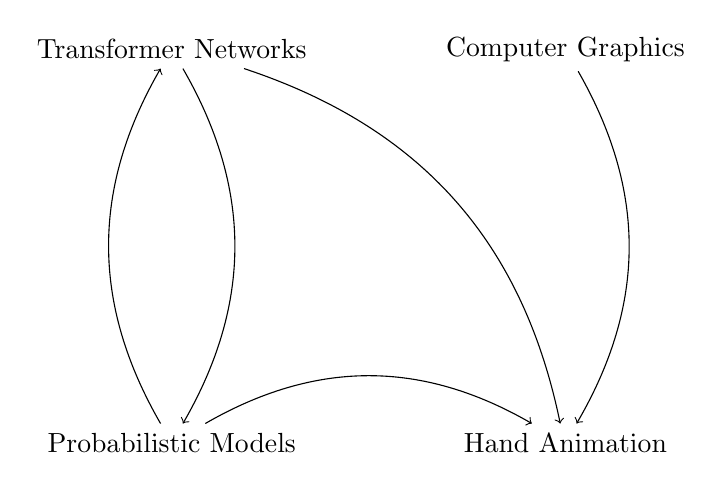
\begin{tikzpicture}
    \tikzstyle{every node}=[node distance=5cm]
    \node (tn) {Transformer Networks};
    \node (pm) [below of=tn] {Probabilistic Models};
    \node (cg) [right of=tn] {Computer Graphics};
    \node (an) [below of=cg] {Hand Animation};

    \draw[->,bend left] (tn) to (pm);
    \draw[->,bend left] (pm) to (tn);
    \draw[->,bend left] (cg) to (an);
    \draw[->,bend left] (pm) to (an);
    \draw[->,bend left] (tn) to (an);
\end{tikzpicture}
\caption[The relationship between the different fields in this thesis]{How learnings and experiments from different fields contribute to each other in this thesis.}
\end{figure}

This thesis introduces concepts and experiments at the intersection of two areas: Deep Learning and Computer Graphics. There are three main areas of focus: Comprehensively introducing a class of neural network models called \textit{transformer} networks; an experiment comparing different sampling orders when predicting data using\textit{auto-regressive} transformer models; and the developement of an application of auto-regressive transformer models for \textit{hand pose modeling}.

\section{Contributions}

Although much of the work done is summarizing others' research and presenting learnings, there are two main novel contributions:
\begin{enumerate}
    \item I present experiments with \textit{dynamically-ordered} auto-regressive sampling, utilising the \textit{permutation-invariance} property of the attention operation in transformer models.
    \item I present a proof-of-concept transformer-based generative model for hand motion prediction, which can be used to predict hand motion at arbitrary target frames, and to predict the joints of a hand in any order within that frame.
\end{enumerate}
These contributions involved training neural networks (see \Cref{fig:context}), in particular transformers, on two datasets - MNIST, and a motion capture dataset of hand motion. The results of these experiments are presented in \Cref{C:a-o-sampling} and \Cref{C:hand-model} respectively.

\begin{figure}
    \centering
    \resizebox{\linewidth}{!}{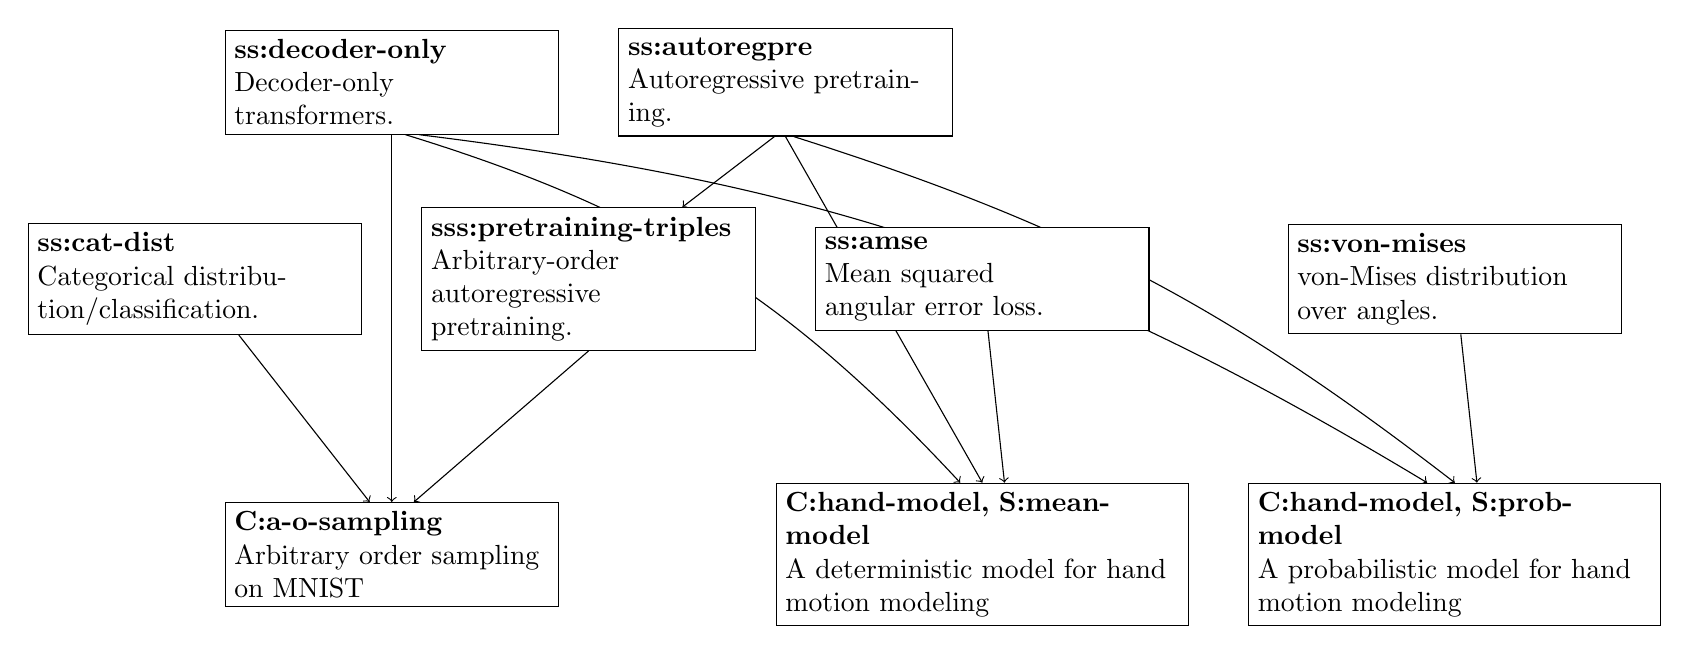
\begin{tikzpicture}
    \pgfdeclarelayer{bg}
    \pgfsetlayers{bg,main}
    \tikzstyle{every node}=[draw,fill=white, text width=4cm,anchor=west, node distance=5cm]
    
    \node (deconly) at (2.5cm, 0) { \textbf{\Cref{ss:decoder-only}} \\ Decoder-only \\ transformers. };
    \node[right of=deconly] (autoregpre) { \textbf{\Cref{ss:autoregpre}} \\ Autoregressive pretraining. };
    
    \node (categorical) at (0, -2.5cm) { \textbf{\Cref{ss:cat-dist}} \\ Categorical distribution/classification. };
    \node[right of=categorical] (aoautoregpre) { \textbf{\Cref{sss:pretraining-triples}} \\ Arbitrary-order \\ autoregressive \\ pretraining. };
    \node[right of=aoautoregpre] (amse) { \textbf{\Cref{ss:amse}} \\ Mean squared \\ angular error loss. };
    \node[right of=amse, node distance=6cm] (vonmises) { \textbf{\Cref{ss:von-mises}} \\ von-Mises distribution over angles. };
    
    \node[below of=categorical,node distance=3.5cm,xshift=2.5cm] (chapter4) {\textbf{\Cref{C:a-o-sampling}} \\ Arbitrary order sampling on MNIST};
    \node[below of=amse,node distance=3.5cm,text width=5cm] (chapter62) {\textbf{\Cref{C:hand-model}, \Cref{S:mean-model}} \\ A deterministic model for hand motion modeling};
    \node[below of=vonmises,node distance=3.5cm,text width=5cm] (chapter63) {\textbf{\Cref{C:hand-model}, \Cref{S:prob-model}} \\ A probabilistic model for hand motion modeling};
    
    \begin{pgfonlayer}{bg}
        \draw[->] ([xshift=-4pt]autoregpre.south) to (aoautoregpre);
        \draw[->] (autoregpre.south) to (chapter62.north);
        \draw[->,bend left=10] ([xshift=3pt]autoregpre.south) to (chapter63.north);
        
        \draw[->] (aoautoregpre.south) to ([xshift=8pt]chapter4.north);
        
        \draw[->] (deconly.south) to (chapter4.north);
        \draw[->, bend left=15] ([xshift=5pt]deconly.south) to ([xshift=-8pt]chapter62.north);
        \draw[->, bend left=12] ([xshift=10pt]deconly.south) to ([xshift=-10pt]chapter63.north);
        
        \draw[->] (categorical) to ([xshift=-8pt]chapter4.north);
        \draw[->] (amse) to ([xshift=8pt]chapter62.north);
        \draw[->] (vonmises) to ([xshift=8pt]chapter63.north);
    \end{pgfonlayer}
\end{tikzpicture}}
    \vspace{1cm}
    \captionsetup{parskip=7pt}
    \caption[Where my work sits.]{The later work in this thesis sits focuses on learning un-labeled sequence data with transformers, in two different domains.

    In \Cref{C:a-o-sampling}, I train a transformer-based probabilistic model which can be used as a gaussian process for predicting pixels on the MNIST dataset.

    In \Cref{C:hand-model}, I train a transformer-based model on the ManipNet hand motion dataset. \Cref{S:mean-model} focuses on a deterministic model, while \Cref{S:prob-model} focuses on a probabilistic model.}
    \label{fig:context}
\end{figure}

\section{Structure}

The structure of the remainder of this thesis is as follows:

\begin{enumerate}
    \item \Cref{C:background} \nameCref{C:background} introduces notation and concepts for neural networks which will be used throughout the thesis.

    \item \Cref{C:transformers} provides an introduction and literature reivew of a class of neural network models called \textit{transformers}, which are a class of models that have become very broadly used in the past few years.

    \item \Cref{C:a-o-sampling} presents a novel method for sampling sequence data in an arbitrary order, including a pretraining task variant, and experiments with this method with transformer models on the MNIST dataset.

    \item \Cref{C:angles-joints-hands} introduces notation and concepts for the problem domain of \textit{hand motion modeling}, including methods for representing and working with joint angles and rotations, and character/hand pose data.

    \item \Cref{C:hand-model} then presents the development of a transformer model for predicting hand pose data and generating animations of hands.

    \item Lastly, \Cref{C:conclusion} summarizes the thesis and discusses future work and reflections.
\end{enumerate}
